\procTitle{Оценка новизны решений в автоматизированной системе распределения грантов}
\procAuthor{Копченко~В.\,К.}
\procEmail{vkkopchenko49@gmail.com}
\procOrganization{СВГУ} \procCity{Магадан}

\makeProcTitleRazdel
\index{k@Копченко~В.\,К.}

В постиндустриальном обществе преобладает инновационный сектор экономики, в котором доминирует высокопроизводительная промышленность, связанная с информационными технологиями. Эти технологии обслуживают потребности государства, бизнеса, организуют социальное взаимодействие, осуществляют информационную поддержку здравоохранения, образования, культуры и иных государственных отраслей. Выделяют следующие наиболее значимые требования к данной области [1, 2]:
\begin{enumerate}[noitemsep]\vspace{-8pt}
      \item адаптацию к постоянно растущему объёму данных;
      \item обеспечение непрерывной работы информационного цикла;
      \item минимизацию ошибок.
\end{enumerate}\vspace{-8pt}

Выполнение данных требований невозможно без надлежащим образом осуществляемого управления на государственном уровне [3]. Например, для первых двух целей в рамках Стратегии развития информационного общества в Российской Федерации на 2017--2030\,гг. [4] было сформулировано направление развития российских информационных и коммуникационных технологий, содержательной основой которого является разработка и обеспечение использования электронно-компонентной базы и программных продуктов российского производства, а также нормативно-правовая и научная базы. Указ Президента РФ №\,203 [5] расширяет круг задач, решаемый интеллектуальными системами, с целью повышения эффективности процессов принятия управленческих решений и минимизации ошибок в таковых.

К последнему классу задач можно отнести распределение ресурсов на основе экспертных оценок в условиях многокритериальности и действующих ограничений, иначе называемое распределением грантов. Данный характер финансирования установлен Указом Президента РФ от 30.01.2019\,г. №\,30 <<О грантах Президента Российской Федерации, предоставляемых на развитие гражданского общества>> [6]. Грантовая система распределения основана на удовлетворении заявок на проектное финансирование. Подобные системы основаны на экспертных оценках, а в свете существующих технологий достойны применения соответствующих средств автоматизации, пренебрежение которыми снижает прозрачность экспертизы, создаёт предпосылки к предвзятому оцениванию в целях собственной выгоды экспертам [7].

В научной публицистике существуют работы, направленные на решение названных проблем. Существующие публикации можно условно разбить на три группы:
\begin{enumerate}[noitemsep]
  \item разработки, направленные на формализацию критериев, что позволит снизить влияние субъективных взглядов эксперта на результат анализа. Примерами таких работ выступают [8--10]. Несмотря на высокий уровень исследований, остаётся открытым вопрос выбора функции свёртки частных показателей, который в настоящее время не решается научным сообществом;
  \item разработки, направленные на формирование экспертных пулов с учётом научно-технического профиля каждого эксперта с динамическим изменением показателей их компетенций в различных отраслях деятельности. Данные рассуждения приведены в работах [11--13]. Следует отметить, что увеличение числа экспертов увеличит затраты на расчёт вышеназванных метрик компетентности, что в большинстве случаев исключает возможность практического использования данного класса разработок;
  \item разработки, направленные на максимальную унификацию критериев оценивания без учёта особенностей, связанных с отраслевой принадлежностью и форматом финансируемого объекта. Яркими примерами служат публикации [14--16]. Данные методы не всегда могут быть применимы, так как у большинства грантооператоров категория применения проекта оценивается согласно перечню приоритетных отраслей экономики, который не поддаётся унификации ввиду отсутствия у многих видов деятельности общих характеристик.
\end{enumerate}

Несмотря на отсутствие готовых концептуальных решений, на основе дальнейшего анализа научных публикаций, в частности [17, 18] можно сделать вывод о сводимости экспертизы любой заявки на проектное финансирование к трём действиям: отраслевой идентификации, анализу уникальности и анализу новизны. Однако, в настоящее время на рынке программных продуктов отсутствуют технические решения для проведения анализа заявки на получение гранта, включающие предложенный комплекс действий, в связи с чем было принято решение о разработке автоматизированной системы распределения грантов (АСРГ), концепция которой сформулирована в работе [19]. Организационно-процессная модель удовлетворения заявки $\Theta$ на грант с отметкой времени \textit{TO BE} представлена следующим кортежем:
\begin{equation}
  \Theta_{TO-BE} = \langle \Psi, P_p, M, Q_p, Q_M, O_M \rangle,
\end{equation}
где $\Psi$~--- множество заявок; $P_p$~--- множество процедур предварительной оценки; $M$~--- процедура экспертной оценки; $Q_p$~--- множество критериев для предварительной оценки; $Q_M$~--- множество критериев для экспертной оценки; $O_M$~--- множество численных оценок. В общем виде схему работы АСРГ можно описать Swimlane-диаграммой (рис.\,1):

Предварительная оценка определяет отраслевую принадлежность проекта согласно исследованию [20]. Величина \textit{r} соответствия заявки \textit{g}-й отрасли знания рассчитывается следующим образом:
\begin{equation}
  r = \text{max}\sum_{\text{c}\,=\,1}^{|\text{G}|}{w_{ij}},
\end{equation}
где G~--- множество отраслей, $\text{G}~= \{g_1, g_2,\dots, g_c \}$, c = |G|, $j=\overline{1,|g_i|}$, $w_{ij}$~--- вес \textit{j}-го терма в~\textit{i}-й отрасли. Термы и веса определены заранее и хранятся в базе данных системы. Данный метод был реализован в рамках конференции [21] и показал высокую эффективность.

\begin{figure}[H]
  \begin{center}
    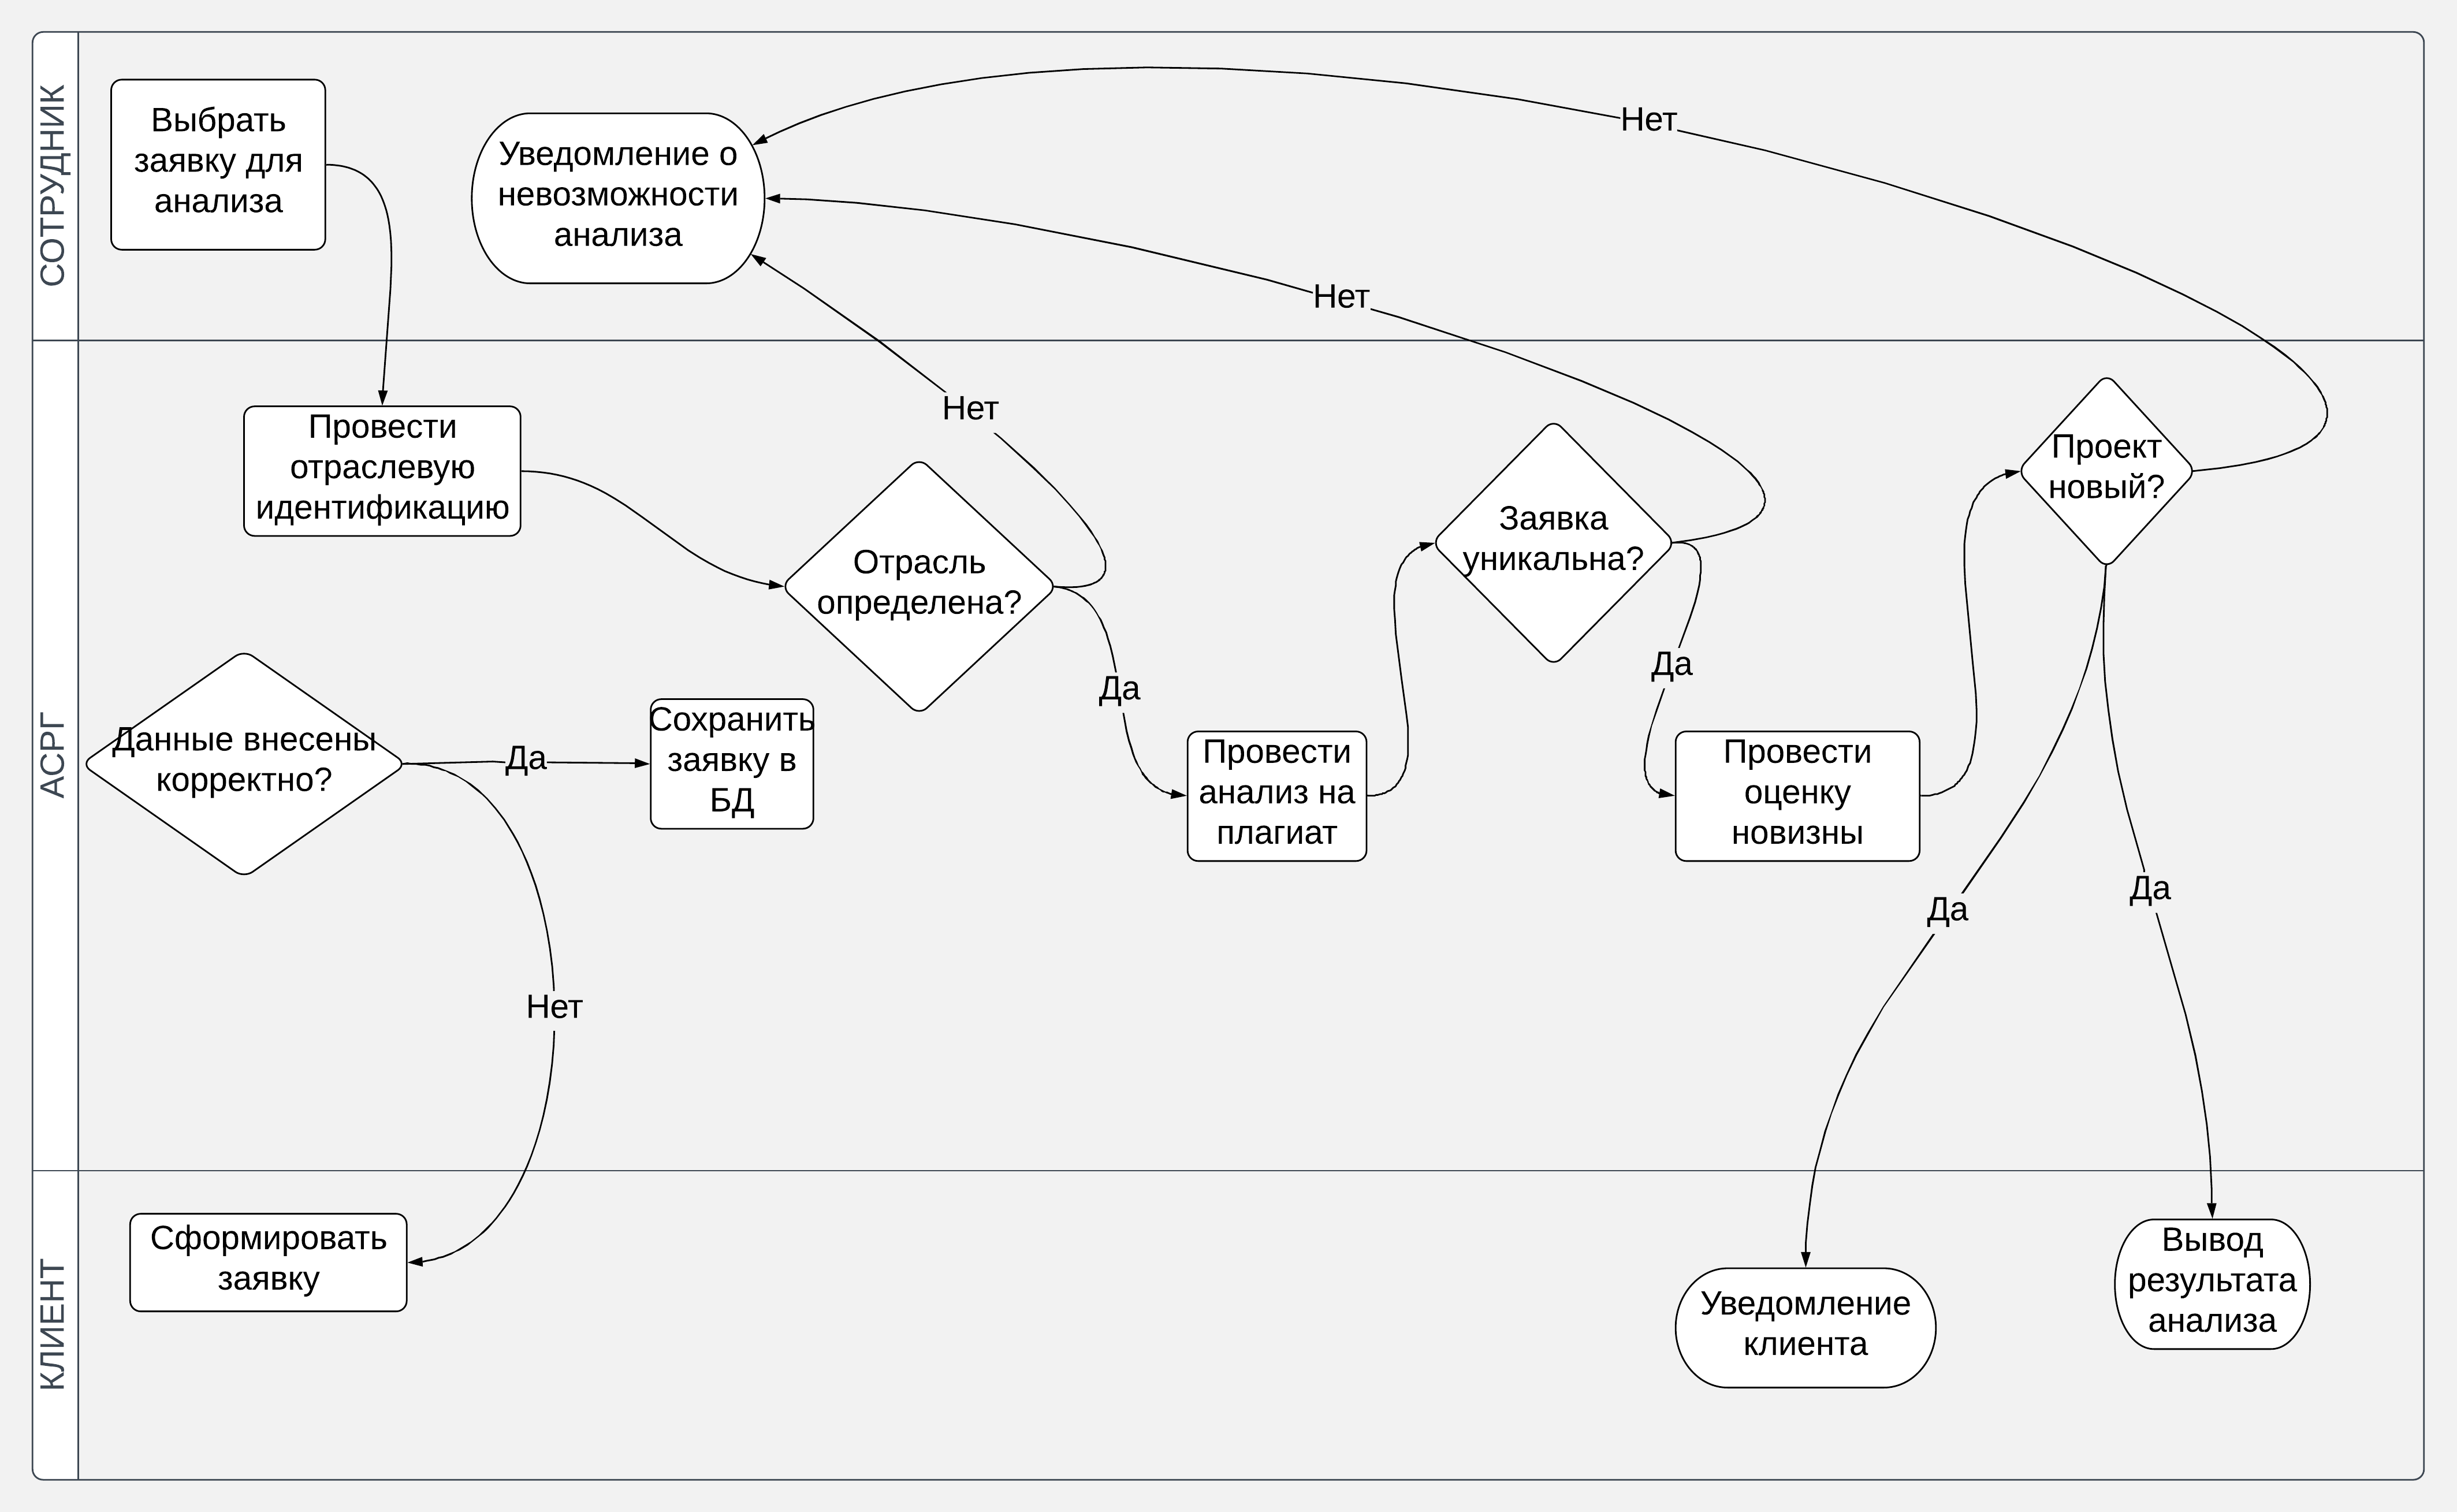
\includegraphics[width=1\textwidth]{authors/kopchenko-fig-1.png}
  \end{center}
  \caption {Swimlane-диаграмма экспертизы АСРГ}

\end{figure}


Экспертная оценка включает в себя анализ заимствований в тексте заявки (плагиат) с~помощью алгоритма шинглов, эффективность которого рассмотрена в работе [22] и оценку новизны предлагаемого проекта. Для реализации данного функционала требуется формализация заявки. Заявка представлена в виде:
\begin{equation}
  R_{eq}= < F, C, V >,
\end{equation}
где \textit{F}~--- краткое описание проекта; \textit{C}~--- детальное описание проекта; \textit{V}~--- атрибуты заявки, определяемые АСРГ. Краткое описание представлено следующей структурой:
\begin{equation}
  F = < F_T, F_S, F_N >,
\end{equation}
где $F_T$~--- наименование проекта; $F_S$~--- краткое описание проекта общими признаками; $F_N$~--- признаки, обеспечивающие новизну решения. Атрибуты АСРГ сопровождаются кортежем:
\begin{equation}
  V = < I, U, H >,
\end{equation}
где \textit{I}~--- отрасль заявки; \textit{U}~--- уникальность заявки; \textit{H}~--- величина новизны проекта.

Оценку новизны можно разделить на три этапа:
\begin{enumerate}[noitemsep]\vspace{-8pt}
    \item поиск прототипа проекта;
    \item поиск отличий проекта от прототипа;
    \item оценка положительного эффекта.
\end{enumerate}\vspace{-8pt}
\clearpage
Прототипом можно считать заявку, у которой величина совпавших с текущей заявкой признаков новизны максимальна:
\begin{equation}
  d_i = \text{max} Sim_j,
\end{equation}
где $Sim_j = F_{N_i} \cap F_{N_j}$ количество совпадений признаков из перечня признаков новизны рассматриваемой \textit{i}-й заявки в списке новшеств документа из архива заявок \textit{Docs}, \textit{d}~--- прототип (заявка). В~случае отсутствия результата можно относительно рассматриваемого множества термов описательной части заявки \textit{С} сопоставить каждому признаку $k_i$ величину $w_i$, называемую весом. В~этом случае прототипом \textit{d} проекта, претендующего на грант, можно считать проект, удовлетворяющий выражению:
\begin{equation}
  d = arg\text{max} \sum_{k=1}^{|Docs|}w_{kj},
\end{equation}
где \textit{k}~--- терм в детальном описании проекта, \textit{w}~--- вес терма, $j=\overline{1,|C|}$.

Данный функционал АСРГ был реализован в виде WEB-приложения на языке php с~использованием WEB-сервера Apache и системой управления базами данных MySQL. Для автоматизации работы с~действиями CRUD и установления базовой защиты была выбрана ORM-библиотека RedBeanPHP, которая отлично зарекомендовала себя как простое в~использовании средство с широким перечнем автоматических операций, вплоть до динамического изменения структуры таблиц и всей базы данных в целом при необходимости, причём прямого вмешательства разработчика в процесс не требуется. Информационная модель предметной области базы данных представлена на рис.\,2.

\begin{figure}[H]
  \begin{center}
    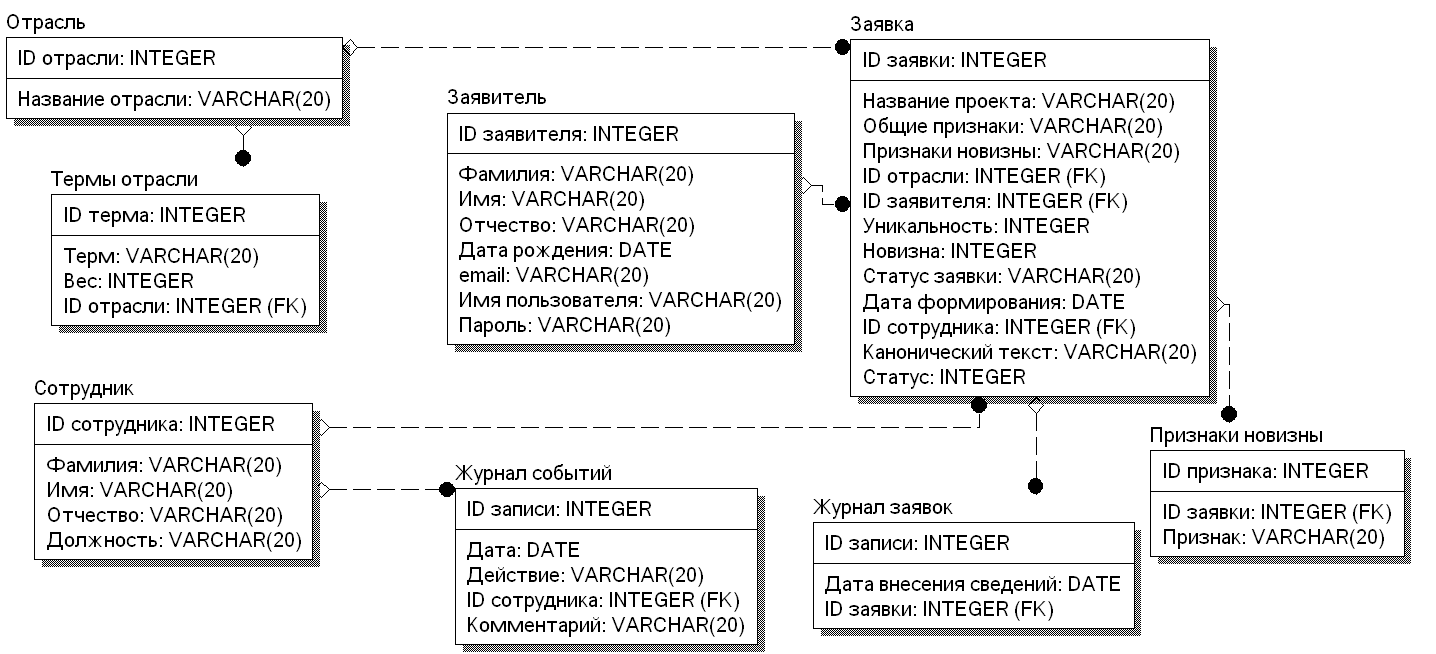
\includegraphics[width=1\textwidth]{authors/kopchenko-fig-2.png}
  \end{center}
  \caption {Информационная модель предметной области базы данных}

\end{figure}


В результате проведённых исследований был разработан программный модуль для оценки новизны проекта, претендующего на получение финансовой поддержки. Работа модуля включает в себя поиск прототипа предлагаемого решения и дальнейший терминологический анализ идентичности при наличии положительного результата. Реализованные средства АСРГ демонстрируют высокую эффективность в анализе отраслевой принадлежности, заимствований и оценке новизны, что предполагает дальнейшие исследования с целью разработки функции свёртки полученных показателей и автоматизации проведения конкурсной процедуры, что позволит минимизировать влияние личных предпочтений эксперта в пользу объективности и скорости анализа заявки.


\begin{thebibliography}{99}
%1

\bibitem{}\BibAuthor{Васин С.\,Г.} Искусственный интеллект в управлении государством // Управление.~--- 2017.~--- №\,3 (17).~--- URL: https://cyberleninka.ru/\-arti\-cle/\-n/iskus\-stven\-nyy-intel\-lekt-v-up\-rav\-lenii-gosu\-dars\-tvom (дата обращения: 16.03.2020).

\bibitem{}\BibAuthor{Вендров\,А.\,М.} Проектирование программного обеспечения экономических информационных систем.~--- М.\,: Финансы и статистика, 2005.~--- 544\,с.

\bibitem{}\BibAuthor{Горчакова\,Е.\,А.} О необходимости унификации критерия отбора проектов кооперации промышленных предприятий в кластере // Известия СПбГЭУ.~--- 2017.~--- №\,5 (107).~--- URL: https://cyberleninka.ru/article/n/o-neobhodimosti-unifikatsii-kriteriya-otbora-proektov-kooperatsii-promyshlennyh-predpriyatiy-v-klastere (дата обращения: 20.02.2020).

\bibitem{}\BibAuthor{Ильин\,И.\,В.} Критерии отбора проектов для их эффективной реализации на условиях проектного финансирования // Финансы и кредит.~--- 2008.~--- №\,35 (323).~--- URL: https://cyberleninka.ru/article/n/kriterii-otbora-proektov-dlya-ih-effektivnoy-realizatsii-na-usloviyah-proektnogo-finansirovaniya-2 (дата обращения: 20.02.2020).

\bibitem{}\BibAuthor{Копченко\,В.\,К., Сироткин\,А.\,В.} Применение систем искусственного интеллекта для распределения грантов предпринимателям Магаданской области // Студенческий: электрон. научн. журн.~--- №\,11 (55).~--- С.\,20--24.

\bibitem{}\BibAuthor{Косоруков\,А.\,А.} Технологии искусственного интеллекта в современном государственном управлении // Социодинамика.~--- 2019.~--- №\,5.~--- С.\,43--58.~--- DOI: 10.25136/2409-7144.2019.5.29714

\bibitem{}III\,Международная научно-практическая конференция <<На перекрестке Севера и Востока (методологии и практики регионального развития)>> / Северо-Восточный государственный университет.~--- 2019.~--- URL: http://svkonf.svgu.ru (дата обращения: 21.02.2020).

\bibitem{}\BibAuthor{Мельник~П.\,Б.} Математическая постановка задачи формирования реестра экспертов // Инноватика и экспертиза.~--- 2014.~--- №\,2 (13).~--- С.~69--81.

\bibitem{}\BibAuthor{Мельник~П.\,Б.} Методика формирования экспертных пулов и групп для проведения экспертно-аналитических исследований // Там же.~--- 2017.~--- №\,1 (19).~--- С.\,39--54.

\bibitem{}\BibAuthor{Мельник~П.\,Б.} Реестр экспертов как система массового обслуживания: модель и параметры входящего потока заявок // Там же.~--- 2018.~--- №\,1 (22).~--- С.\,67--78.

\bibitem{}\BibAuthor{Морозова\,Т.\,В.} Экспертные технологии в оценке инновационных проектов // Известия ЮФУ. Технические науки.~--- 2011.~--- №\,11.~--- URL: https://cyberleninka.ru/article/n/ekspertnye-tehnologii-v-otsenke-innovatsionnyh-proektov (дата обращения: 20.02.2020).

\bibitem{}\BibAuthor{Марон~А.\,И., Марон~М.\,А.} Метод конкурсного отбора проектов // Открытое образование.~--- 2011.~--- №\,2.~--- URL: https://cyberleninka.ru/article/n/metod-konkursnogo-otbora-proektov (дата обращения: 20.02.2020).

\bibitem{}\BibAuthor{Новикова\,Т.\,Г.} Теоретические основы экспертизы инновационной деятельности в образовании~: автореф. дис. $\dots$ д-ра пед. наук.~--- Москва, 2006.~--- 47\,с.


\bibitem{}\BibAuthor{Семиглазов\,В.\,А.} Развитие методики отбора инновационных проектов в условиях полной неопределенности // Инновации.~--- 2006.~--- №\,11.~--- URL: https://cyberleninka.ru/article/n/razvitie-metodiki-otbora-innovatsionnyh-proektov-v-usloviyah-polnoy-neopredelennosti (дата обращения: 20.02.2020).

\bibitem{}\BibAuthor{Сироткин\,А.\,В, Копченко\,В.\,К.} Концепция разработки автоматизированной системы распределения грантов // EurasiaScience~: сб. статей XXI междунар. науч.-практ. конф.~--- М.\,: Науч.-издат. центр <<Актуальность.рф>>, 2019.~--- С.\,107--109.

\bibitem{}\BibAuthor{Сироткин\,А.\,В., Старикова\,О.\,А.} Отраслевая идентификация заявок в автоматизированной экспертной системе распределения грантов // Современные наукоёмкие технологии.~--- 2019.~--- №\,7.~--- С.\,99--103.

\bibitem{}Указ Президента РФ от 09.05.2017~г. №~203 <<О\,Стратегии развития информационного общества в Российской Федерации на 2017--2030 годы>>~// Консультант Плюс.~--- URL: http://www.consultant.ru/document/cons\_doc\_LAW\_216363/ (дата обращения: 16.03.2020).

\bibitem{}Указ Президента Российской Федерации от 10.10.2019~г. №~490 <<О развитии искусственного интеллекта в Российской Федерации>>~// Консультант Плюс.~--- URL: http://www.consultant.ru/document/cons\_doc\_LAW\_335184/ (дата обращения: 16.03.2020).

\bibitem{}Указ Президента РФ от 30.01.2019~г. №~30 <<О грантах Президента Российской Федерации, предоставляемых на развитие гражданского общества>>~// Законы, кодексы и нормативно-правовые акты в Российской Федерации.~--- URL: https://legalacts.ru/doc/ukaz-prezidenta-rf-ot-30012019-n-30-o-grantakh/\#100014 (дата обращения: 16.03.2020).


\bibitem{}\BibAuthor{Шушкевич~Н.\,А., Мохов~А.\,И., Крупский~А.\,Ю., Нургазиева~А.\,С.} Экспертиза проектов на основе информационной модели // Вестник евразийской науки.~--- 2010.~--- №\,4.~--- URL: https://cyberleninka.ru/article/n/ekspertiza-proektov-na-osnove-informatsionnoy-modeli (дата обращения: 20.02.2020).


\bibitem{}\BibAuthor{Ясенев\,В.\,Н.} Информационные системы и технологии в экономике / 3-е изд., перераб. и доп.~--- М.\,: ЮНИТИ, 2012.~--- 560\,с.

\bibitem{}\BibAuthor{Broder\,A.} Identifying and Filtering Near-Duplicate Documents, COM’00 // Proceedings of the 11th Annual Symposium on Combinatorial Pattern Matching.~--- 2000.~--- P.\,1--10.
\end{thebibliography}
\thispagestyle{empty}
